\hypertarget{elipsoide}{\subsection{Elipsoide en la aproximación cuasiestática}}
Las secciones transversales de extinción, absorción y esparcimiento para distribuciones arbitrarias de cargas y corrientes confinadas a distancias cortas respecto al punto de observación fueron estudiadas en la sección anterior. En esta sección se estudia el caso particular del esparcimiento de luz por cargas y corrientes iluminadas por una onda plana electromagnética y confinadas en un elipsoide centrado en el origen, con semiejes $a,b,c$ alineados con los ejes $\uvec{x},\uvec{y},\uvec{z}$ respectivamente, y dimensiones tales que $\lambda\gg a>b>c$ [ver Fig. \ref{elipse}], donde $\lambda$ se relaciona con el vector de onda como $k=2\pi\sqrt{\epsilon_m}/\lambda$. A diferencia de la sección anterior, no se cuenta con simetría esférica, sin embargo es posible calcular una solución analítica, aproximada, al emplear las coordenadas elipsoidales confocales\footnote{Existen diversas definiciones que pueden revisarse en la Ref. \cite{ConfocalEllip}, sin embargo, se emplea la proporcionada en la Ref.~\cite{Arfken}. }, que describen la superficie del elipsoide como \cite{ConfocalEllip}
\begin{equation}
	\frac{x^2}{a^2-u}+\frac{y^2}{b^2-u}+\frac{z^2}{c^2-u}=1,
	\label{elipsoide2}
\end{equation}
 donde debe determinarse el valor del parámetro $u$. La Ec. (\ref{elipsoide2}) es una ecuación de tercer grado para $u$, por lo que las soluciones (reales) son un conjunto de tres valores $\{\xi,\eta,\zeta\}$ tales que\footnote{La función $f(u)=x^2/(a^2-u)+y^2/(b^2-u)+z^2/(c^2-u)-1$ resulta ser continuamente diferenciable en el dominio $(-\infty, c^2)\cap (c^2, b^2)\cap (b^2, a^2)$ y estrictamente creciente en cada intervalo que lo compone, de tal forma que, al calcular los límites en cada extremo de los intervalos, se concluye que existe exactamente una raíz en cada intervalo.}
\begin{equation}
	-\infty<\xi<c^2<\eta<b^2<\zeta<a^2,
\end{equation}
que corresponden a tres formas cuádricas con focos en común [ver Fig. \ref{Quadrics}]. Las coordenadas elipsoidales confocales se relacionan con las coordenadas cartesianas mediante el siguiente sistema de ecuaciones escrito en forma matricial
%
	\begin{equation*}
		\begin{pmatrix}
			\frac{1}{a^2+\xi} & \frac{1}{b^2+\xi} & \frac{1}{c^2+\xi}\\
			\frac{1}{a^2+\eta} & \frac{1}{a^2+\eta} & \frac{1}{a^2+\eta}\\
			\frac{1}{a^2+\zeta} & \frac{1}{a^2+\zeta} & \frac{1}{a^2+\zeta}\end{pmatrix}\begin{pmatrix}
			x^2\\
			y^2\\
			z^2
		\end{pmatrix}=\begin{pmatrix}
			1\\
			1\\
			1
		\end{pmatrix},
	\end{equation*}
%	
cuya solución está dada por las expresiones
\begin{align}
	x^2&=\frac{(a^2+\xi)(a^2+\eta)(a^2+\zeta)}{(b^2-a^2)(c^2-a^2)},\label{x_elips}\\
	y^2&=\frac{(b^2+\xi)(b^2+\eta)(b^2+\zeta)}{(a^2-b^2)(c^2-b^2)},\label{y_elips}\\
	z^2&=\frac{(c^2+\xi)(c^2+\eta)(c^2+\zeta)}{(a^2-c^2)(b^2-c^2)}. \label{z_elips}    
\end{align}
A partir del sistema de ecuaciones dado por las Ecs. (\ref{x_elips}), (\ref{y_elips}) y (\ref{z_elips}), se observa que cuando $\xi$ es constante, se obtiene un elipsoide. De esta forma, la superficie de la partícula a estudiar se tiene cuando $\xi=0$. Mientras que si $\eta$ es constante, se obtiene un hiperboloide de una hoja y cuando $\zeta$ es constante se tiene un hiperboloide de dos hojas. Cada punto ($x,y,z$) tiene una correspondencia única con ($\xi,\eta,\zeta$), pero la transformación inversa no es biyectiva, ya que cada ($\xi,\eta,\zeta$) se asocia a ocho puntos simétricos respecto a los ejes ($x,y,z$) \cite{Cambdrige}. \\

\begin{figure}[H]
	\centering
	\sidesubfloat[][]{\vspace{10cm}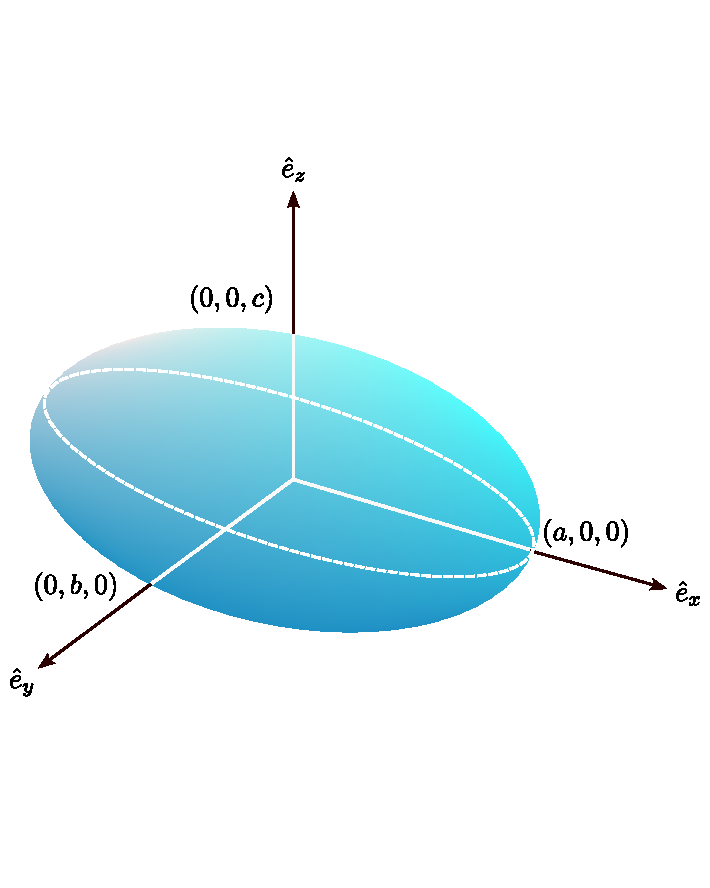
\includegraphics[width=0.45\textwidth]{../../Figuras/ellipsoid}\label{elipse}}
	\sidesubfloat[][b]{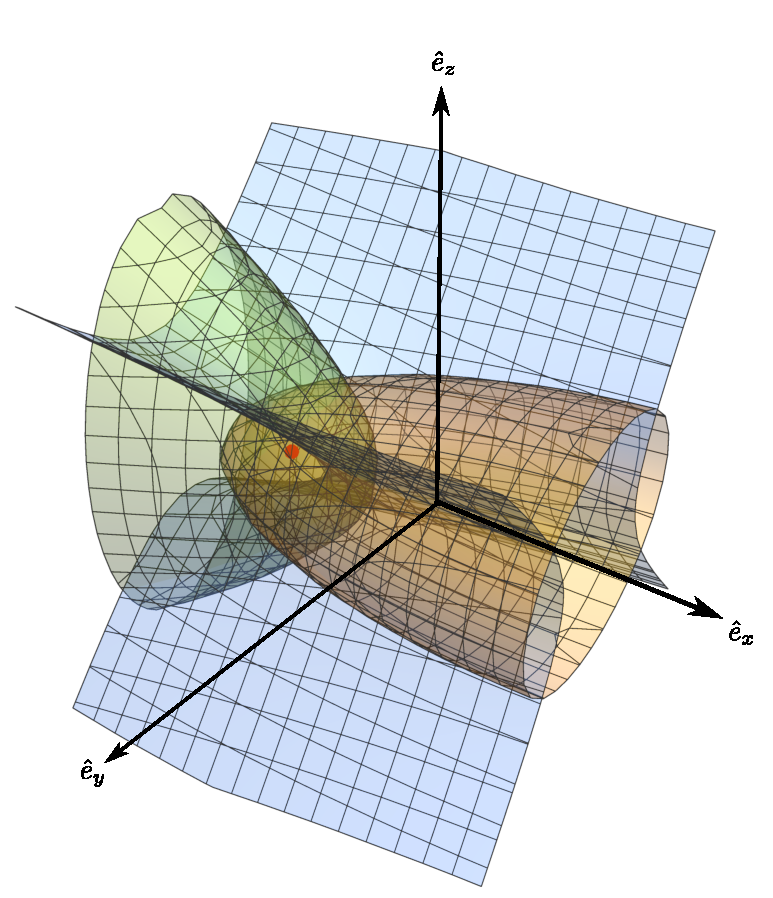
\includegraphics[width=0.4\textwidth]{../../Figuras/quadraticonfo}\label{Quadrics}}
	\caption{\textbf{a)} Elipsoide centrado en el origen, con semiejes $a, b, c$ tales que $a > b > c.$   \textbf{b)} Superficies confocales. Hiperboloide de una hoja (superficie azul) con $u=0.8$, hiperboloide de dos hojas (superficie verde) con $u=0.5$ y elipsoide (superficie naranja) con $u=0.1$. Todas las superficies poseen semiejes con valores $a=1, b=0.8$ y $c=0.6$. El punto rojo representa uno de los focos en común localizado en (-0.8,0,0).}
	\label{ConfocalQuadrics}
\end{figure}



En el problema de esparcimento de luz en el límite cuasiestático (o sin retardo) se resuelve la ecuación de Laplace para el potencial eléctrico, que  en un sistrema coordenado arbitrario se escribe como \cite{Arfken}
\begin{equation}
	\nabla^2\phi=\frac{1}{h_1h_2h_3}\left[\frac{\partial}{\partial q_1}\left(\frac{h_2h_3}{h_1}\frac{\partial\phi}{\partial q_1}\right)+\frac{\partial}{\partial q_2}\left(\frac{h_3h_1}{h_2}\frac{\partial\phi}{\partial q_2}\right)+\frac{\partial}{\partial q_3}\left(\frac{h_1h_2}{h_3}\frac{\partial\phi}{\partial q_3}\right)\right],
	\label{laplaciano}    
\end{equation}
donde $\phi$ es una función escalar, y  $h_i$ con $i=1,2,3$ los factores de escala que, para coordenadas elipsoidales se asocian como $1\rightarrow\xi, 2\rightarrow\eta$ y $3\rightarrow\zeta,$ y se determinan al hacer un cambio de base de coordenadas cartesianas a elipsoidales. Estos factores de escala están dados por \cite{Arfken}
\begin{equation}
	h_i=\Big|\frac{\partial \Vec{r}}{\partial q_i}\Big|=\sqrt{\left(\frac{\partial x}{\partial q_i}\right)^2+\left(\frac{\partial y}{\partial q_i}\right)^2+\left(\frac{\partial z}{\partial q_i}\right)^2},
\end{equation} 
que para coordenadas elipsoidales, considerando la variación en la dirección $x$, empleando la Ec. (\ref{x_elips}), se tiene que \begin{align*}
	\frac{\partial x}{\partial \xi}&=\frac{1}{2}\left(\frac{(a^2+\xi)(a^2+\eta)(a^2+\zeta)}{(b^2-a^2)(c^2-a^2)}\right)^{-1/2}\frac{\partial}{\partial \xi}\left(\frac{(a^2+\xi)(a^2+\eta)(a^2+\zeta)}{(b^2-a^2)(c^2-a^2)}\right)\nonumber\\
	&=\frac{1}{2}\frac{1}{a^2+\xi}\sqrt{\frac{(a^2+\xi)(a^2+\eta)(a^2+\zeta)}{(b^2-a^2)(c^2-a^2)}}\nonumber\\
	&=\frac{1}{2x}\frac{\partial x^2}{\partial\xi},
\end{align*}
por tanto,
\begin{equation*}
	\frac{\partial x}{\partial \xi}=\frac{1}{2}\frac{x}{(a^2+\xi)}.
\end{equation*}
Empleando las Ecs. (\ref{y_elips}) y (\ref{z_elips}) para $y$ y $z$, respectivamente, se obtiene
\begin{align*}
	\frac{\partial y}{\partial \xi}&=\frac{1}{2y}\frac{\partial y^2}{\partial\xi}=\frac{1}{2}\frac{y}{(b^2+\xi)},\\
	\frac{\partial z}{\partial \xi}&=\frac{1}{2z}\frac{\partial z^2}{\partial\xi}=\frac{1}{2}\frac{z}{(c^2+\xi)}.
\end{align*}
De esta forma, el cuadrado del primer factor de escala $h_1$ es
\begin{equation}
	h_1^2=\frac{1}{4}\left[\frac{x^2}{(a^2+\xi)^2}+\frac{y}{(b^2+\xi)^2}+\frac{z}{(c^2+\xi)^2}\right];
	\label{h1}
\end{equation}
y por economía, se define a la función $g(u)=(u-\xi)(u-\eta)(u-\zeta)$, que permite reescribir la Ec. (\ref{elipsoide2}) como
\begin{equation}
	1-\frac{x^2}{a^2+u}-\frac{y^2}{b^2+u}-\frac{z^2}{c^2+u}=\frac{g(u)}{(a^2+u)(b^2+u)(c^2+u)},
\end{equation}
donde $g(u)$ es una función cúbica con tres raíces reales dentro del rango descrito por los límites de cada variable, y al  derivarla con respecto de $u$ se obtiene
\begin{align}
	\frac{x^2}{(a^2+u)^2}+\frac{y^2}{(b^2+u)^2}+\frac{z^2}{(c^2+u)^2}&=\frac{g(u)}{[f(u)]^2}\left[\frac{1}{u-\xi}+\frac{1}{u-\zeta}+\frac{1}{u-\eta}-\left(\frac{1}{a^2+u}+\frac{1}{b^2+u}+\frac{1}{c^2+u}\right)\right],
\end{align}
con 
\begin{equation}
	f(u)=\sqrt{(a^2+u)(b^2+u)(c^2+u)},  
\end{equation}
por medio del cual se puede reescribir al primer factor de escala de la Ec. (\ref{h1}) como
\begin{align*}
	h_1^2&=\frac{1}{4}\frac{g(u)}{[f(u)]^2}\left[\frac{(u-\zeta)(u-\eta)+(u-\xi)(u-\eta)+(u-\xi)(u-\zeta)}{g(u)}-\left(\frac{1}{a^2+u}+\frac{1}{b^2+u}+\frac{1}{c^2+u}\right)\right].    
\end{align*}
Dado que $\xi$ es una raíz de $g(u)$, entonces $g(u)=0$, por lo que el factor de escala $h_1$ es
\begin{equation}
	h_1=\frac{\sqrt{(\xi-\eta)(\xi-\zeta)}}{2f(\xi)}.
	\label{h1_1}
\end{equation}
Mediante un proceso análogo, se tiene que \cite{Arfken}
\begin{equation}
	h_2=\frac{\sqrt{(\eta-\xi)(\eta-\zeta)}}{2f(\eta)}\hspace{0.5cm}\mbox{y}\hspace{0.5cm}
	h_3=\frac{\sqrt{(\zeta-\xi)(\zeta-\eta)}}{2f(\zeta)}.
	\label{h2yh3}
\end{equation}
Sustituyendo las Ecs. (\ref{h1}) y (\ref{h2yh3}) en la Ec. (\ref{laplaciano}), y simplificando se obtiene
\begin{align*}
	\nabla^2\phi=\frac{4}{\Upsilon}\left[(\eta-\zeta)f(\xi)\frac{\partial}{\partial\xi}\left(f(\xi)\frac{\partial\phi}{\partial\xi}\right)+(\zeta-\xi)f(\eta)\frac{\partial}{\partial\eta}\left(f(\eta)\frac{\partial\eta}{\partial\eta}\right)+(\xi-\zeta)f(\zeta)\frac{\partial}{\partial\zeta}\left(f(\zeta)\frac{\partial\phi}{\partial\zeta}\right)\right],
\end{align*}
donde a $\Upsilon$ se le conoce como el valor absoluto del determinante funcional \cite{Kellog}
\begin{equation}
	\Upsilon=(\xi-\eta)(\zeta-\xi)(\eta-\zeta).
\end{equation}
Como resultado de lo anterior, la ecuación de Laplace en coordenadas elipsoidales se reescribe como
\begin{equation}
	\nabla^2\phi=(\eta-\zeta)f(\xi)\frac{\partial}{\partial\xi}\left(f(\xi)\frac{\partial\phi}{\partial\xi}\right)+(\zeta-\xi)f(\eta)\frac{\partial}{\partial\eta}\left(f(\eta)\frac{\partial\eta}{\partial\eta}\right)+(\xi-\eta)f(\zeta)\frac{\partial}{\partial\zeta}\left(f(\zeta)\frac{\partial\phi}{\partial\zeta}\right)=0.
	\label{laplaceplisoidal}
\end{equation}
Una de las formas por la cual se puede resolver la ecuación anterior es mediante el método de reducción de orden, el cual proporciona una solución linealmente independiente a partir de otra conocida con anterioridad \cite{Braun}. En este contexto, $\phi$ corresponde a la solución de dicha ecuación que está determinada por la forma del campo incidente y cumple las condiciones de frontera. \\


El potencial eléctrico solución a la Ec. (\ref{laplaceplisoidal}) hereda la simetría del sistema de interés, el cual consiste en un elipsoide homogéneo iluminado por un campo eléctrico incidente uniforme alineado a lo largo del eje $\uvec{z}$. Por tanto,  a cada punto del espacio descrito por las coordenadas elipsoidales le corresponden ocho puntos en las coordenadas cartesianas. Es decir, las propiedades de simetría del sistema en el potencial eléctrico son:
\begin{equation}
    \phi(x,y,z)=\phi(-x,y,z)=\phi(x,-y,z)=\phi(-x,-y,z),
\end{equation}
\begin{equation}
    \phi(x,y,-z)=\phi(-x,y ,-z)=\phi(x,-y,-z)=\phi(-x,-y,-z),
\end{equation}
donde $z$ es positiva. Entonces, sólo se tiene que considerar el potencial en dos octantes: uno con $z$ positivo y otro con $z$ negativo. \\

Dado que se quiere determinar el potencial eléctrico producido de la interacción entre el campo eléctrico externo y la distribución de cargas y corrientes confinadas en un elipsoide, se propone dividir el problema en dos regiones espaciales: al exterior y al interior del elipsoide, de modo que el potencial total se puede expresar como la contribución del potencial en el exterior del elipsoide $\phi_{ext}$  y la contribución en el interior de éste $\phi_{int}$. Asimismo, se propone descomponer al potencial $\phi_{ext}$ en una contribución de la onda plana incidente $\phi_0$ y en otra de perturbación $\phi_f$, la cual correspondería al campo eléctrico esparcido por la partícula
\begin{equation}
	\phi_{ext}(\xi,\eta,\zeta)=\phi_0(\xi,\eta,\zeta)+\phi_f(\xi,\eta,\zeta),    
\end{equation}
donde, de acuerdo con la expresión para $z$ en la Ec. (\ref{z_elips}),
\begin{equation}
	\phi_0=-E_0 r\cos\theta=-E_0 z=-E_0\left[\frac{(c^2+\xi)(c^2+\eta)(c^2+\zeta)}{(a^2-c^2)(b^2-c^2)}\right]^{1/2}.
	\label{pot_0}
\end{equation}

Al considerar las condiciones de frontera en el sistema en dos límites: a distancias muy lejanas del elipsoide y en la interfaz entre el medio y el elipsoide, debido al teorema de unicidad \cite{Griffiths}, el problema queda totalmente determinado. Para distancias lo suficientemente lejanas a la partícula, es decir, cuando $\xi\gg a^2$, al factorizar $\xi$ de  la Ec. (\ref{x_elips}), se obtiene
\begin{equation*}
    \frac{x^2}{a^2/\xi+1}+\frac{y^2}{b^2/\xi+1}+\frac{z^2}{c^2/\xi+1}=\xi,
\end{equation*}
donde
\begin{equation*}
    \lim_{\xi\rightarrow\infty}\left(\frac{x^2}{a^2/\xi+1}+\frac{y^2}{b^2/\xi+1}+\frac{z^2}{c^2/\xi+1}\right)=x^2+y^2+z^2=r^2,
\end{equation*}
entonces, $\xi \simeq r^2$ en el límite asintótico. Asimismo, en esta aproximación el potencial de perturbación es despreciable, por lo que 
\begin{equation}
\lim_{\xi\rightarrow\infty}\phi_f=0
\label{limitephi_p}.
\end{equation}
Al considerar $\phi_{int}$ y $\epsilon_{int}$ el potencial y la permitividad eléctrica en el interior del elipsoide, y las mismas cantidades $\phi_{ext}$ y $\epsilon_{ext}$ para el exterior de éste, como el potencial es continuo en la superficie del elipsoide y la componente perpendicular a la superficie del elipsoide del campo de desplazamiento eléctrico $\Vec{D}$ por ausencia de cargas externas también \cite{Griffiths}
\begin{subequations}
\label{condicionesfrontera}
\begin{align}
    \phi_{int}|_{\xi=0}&=\phi_{ext}|_{\xi=0}\label{cf1},\\
    \epsilon_{int}\frac{\partial \phi_{int}}{\partial \xi}\Big |_{\xi=0}&=
    \epsilon_{ext}\frac{\partial \phi_{ext}}{\partial \xi}\Big |_{\xi=0}\label{cf2},
\end{align}
\end{subequations}
en donde se emplea la relación constitutiva $\Vec{D}=\epsilon\Vec{E}$ y que $E_{int}^{\perp}=-\partial \phi_{int} /\partial \xi$.\\


Reescribiendo los potenciales $\phi_{int}$ y $\phi_0$ de la forma
\begin{align}
    \phi(\xi,\eta,\zeta)&=F(\xi)[(c^2+\eta)(c^2+\zeta)]^{1/2}, 
    \label{phi0 con F}
\end{align}
donde $F(\xi)$ es una función cuya única variable independendiente es $\xi$, se obtiene que, para que satisfagan la Ec. (\ref{laplaceplisoidal}), se tiene que cumplir 
\begin{equation}
  (\eta-\zeta)[(c^2+\zeta)(c^2+\eta)]^{1/2}\left[f(\xi)\frac{\text{d}}{\text{d}\xi}\left(f(\xi)\frac{ \text{d} F(\xi)}{\text{d}\xi}\right)-\frac{1}{4}F(\xi)(a^2+b^2+2\xi)\right]=0,
\end{equation}
lo cual es equivalente a resolver
\begin{equation}
    f(\xi)\frac{\text{d}}{\text{d}\xi}\left(f(\xi)\frac{ \text{d} F(\xi)}{\text{d}\xi}\right)-\left(\frac{a^2+b^2}{4}+\frac{\xi}{2}\right)F(\xi)=0.
    \label{ecsimpli}
\end{equation}
La ecuación anterior es una ecuación diferencial ordinaria lineal de segundo orden, con dos soluciones no triviales linealmente independientes. Una de estas soluciones es
\begin{equation}
    F_1(\xi)=(c^2+\xi)^{1/2},
    \label{F1}
\end{equation}
y la segunda solución se obtiene mediante el método de reducción de orden. Como $F_1(\xi)$ es solución de la Ec. (\ref{laplaceplisoidal}), se propone una segunda solución dada por $F_2(\xi)=v(\xi)F_1(\xi)$ donde $v(\xi)$ se determina al sustituir dicha solución en la ecuación diferencial dada, reduciéndola a una ecuación de primer orden donde la variable dependiente será $v$. Derivando la ecuación anterior respecto a $\xi$
\begin{align*}
    \frac{\text{d}F_2(\xi)}{\text{d}\xi}&=F_1(\xi)\frac{\text{d}v(\xi)}{\text{d}\xi}+v(\xi)\frac{F_1(\xi)}{\text{d}\xi},\\
    \frac{\text{d}^2F_2(\xi)}{\text{d}\xi^2}&=F_1(\xi)\frac{\text{d}^2v(\xi)}{\text{d}\xi^2}+2\frac{\text{d}v(\xi)}{\text{d}\xi}\frac{\text{d}F_1(\xi)}{\text{d}\xi}+v(\xi)\frac{\text{d}^2F_1(\xi)}{\text{d}\xi^2},
\end{align*}
y sustituyendo las derivadas anteriores en la Ec. (\ref{F1}), y simplificando, se obtiene
\begin{equation*}
    f^2(\xi)F_1(\xi)\frac{\text{d}^2v(\xi)}{\text{d}\xi^2}+\frac{\text{d}v(\xi)}{\text{d}\xi}\left[f(\xi)F_1(\xi)\frac{\text{d}f(\xi)}{\text{d}\xi}+2f^2(\xi)\frac{\text{d}F_1(\xi)}{\text{d}\xi}\right]=0.
\end{equation*}
Haciendo el cambio de variable $V(\xi)=dv(\xi)/d\xi$ y reordenando términos resulta que
\begin{equation}
    \frac{1}{V(\xi)}\frac{\text{d}V(\xi)}{\text{d}\xi}=-\frac{1}{f^2(\xi)F_1(\xi)}\left[f(\xi)F_1(\xi)\frac{\text{d}f(\xi)}{\text{d}\xi}+2f^2(\xi)\frac{\text{d}F_1(\xi)}{\text{d}\xi}\right],
    \label{integralindef}
\end{equation}
donde al realizar la integral indefinida de la Ec. (\ref{integralindef}) da como resultado
\begin{align*}
    \ln[V(q)]=-\ln[F_1^2(q)f(q)],
\end{align*}
entonces,
\begin{equation*}
    \frac{\text{d}v(q)}{\text{d}q}=\frac{1}{F_1^2(q)f(q)}.
\end{equation*}
Como $\text{d}v(q)/\text{d}q$ es distinto de cero,  $v(q)$ es distinto de una constante. Integrando lo anterior se tiene que
\begin{equation*}
    v(\xi)=\int_{\xi}^{\infty}\frac{\text{d}q}{F_1^2(q)f(q)},
\end{equation*}
por lo tanto, 
\begin{equation}
  F_2(\xi)=F_1(\xi)\int_{\xi}^{\infty}\frac{\text{d}q}{F_1^2(q)f(q)}.
  \label{F2}
\end{equation}
Al escribir explícitamente el integrando, usando las Ecs. (\ref{F1}) y (\ref{F2}), y haciendo una integración por partes con $u=1/(a^2+q)^{1/2}$ y $\text{d}v=1/[(c^2+q)^{3/2}(b^2+q)^{1/2}]$, se obtiene
\begin{align}
    F_2(\xi)&=F_1(\xi)\int_{\xi}^{\infty}\frac{\text{d}q}{(c^2+q)[(a^2+q)(b^2+q)(c^2+q)]^{1/2}}\nonumber\\
    &=\frac{F_1(\xi)}{c^2-b^2}\left[\frac{b^2+q}{(a^2+q)(c^2+q)}\right]^{1/2}\Bigg|_\xi^{\infty}-\int_\xi^{\infty}\sqrt{\frac{b^2+q}{c^2+q}}\frac{\text{d}q}{(c^2-b^2)(a^2+q)^{3/2}}.
\end{align}
Reescribiendo la segunda integral
\begin{equation}
	\int_\xi^{\infty}\frac{\sqrt{\frac{b^2+q}{a^2+q}}\sqrt{\frac{b^2+q}{a^2+q}}\sqrt{a^2-c^2}\:\text{d}q}{\sqrt{a^2-c^2}(c^2-b^2)\sqrt{\frac{c^2+q}{a^2+q}}\sqrt{\frac{b^2+q}{c^2+q}}(a^2+q)^{3/2}\sqrt{\frac{c^2+q}{a^2+q}}},\label{eliptic}
\end{equation}
y considerando que
\begin{equation*}
	\frac{\text{d}}{\text{d}q}\left\{E\left[\mbox{arcsen}\left(\frac{\sqrt{a^2-c^2}}{\sqrt{a^2+q}}\right)\Bigg|\frac{a^2-b^2}{a^2-c^2}\right]\right\}=-\frac{\sqrt{\frac{b^2+q}{a^2+q}}\sqrt{a^2-c^2}}{(a^2+q)^{3/2}\sqrt{\frac{c^2+q}{a^2+q}}}
\end{equation*}
al sustituir en la Ec. (\ref{eliptic}) y haciendo uso del teorema fundamental del cálculo, se obtiene que la segunda solución a la Ec. (\ref{ecsimpli}) es 
\begin{align}
    F_2(\xi)&=\frac{2F_1(\xi)}{c^2-b^2}\Bigg\{\left[\frac{b^2+q}{(a^2+q)(c^2+q)}\right]^{1/2}-\frac{1}{(a^2-c^2)^{1/2}}E\left(\mbox{arcsen}\left(\frac{\sqrt{a^2-c^2}}{a^2+q}\right)\Bigg|\frac{a^2-b^2}{a^2-c^2}\right)\Bigg\}\Bigg|_\xi^{\infty},
    \label{F2_xi}
\end{align}
donde $E(\phi|m)$ es una integral elíptica de segundo tipo definida como  \cite{Abramowitz}
\begin{equation}
    E(x|\kappa)=\int_{0}^x\frac{\sqrt{1-\kappa^2t^2}}{1-t^2}\text{d}t,\hspace{1cm}0\leq m\leq 1,
\end{equation}
donde el módulo angular es $\beta=\mbox{arcsen}\:\kappa$ y $\kappa$ es la excentricidad. En el primer límite de integración ($\infty$) de $F_2(\xi)$ en la Ec. (\ref{F2_xi}), al evaluar se obtiene que el primer sumando es cero, y en el segundo límite la función arcoseno es cero. De ésta forma, la parte angular de la integral es cero, es decir, $E(0|m)=0$. En consecuencia, considerando la definición de $F_1$ en la Ec. (\ref{F1}) se tiene que $F_1$ y $F_2$ cumplen

\begin{equation}
    \lim_{\xi \to 0}F_1(\xi)=c\hspace{1cm}\mbox{y}\hspace{1cm} \lim_{\xi \to \infty}F_2(\xi)=0.
\end{equation}
De esta forma, considerando que $F_1$ no satisface la condición impuesta sobre $\phi_f$ en la Ec. (\ref{limitephi_p}) y que necesariamente el potencial dentro de la partícula debe de ser finito, lo cual $F_2$ no satisface, los potenciales $\phi_{int}$ y $\phi_f$, propuestos como en la Ec. (\ref{phi0 con F}), están dados por
\begin{align}
    \phi_{int}&=C_1F_1(\xi)[(c^2+\eta)(c^2+\zeta)]^{1/2}\label{phi_int},\\
    \phi_f&=C_2F_2(\xi)[(c^2+\eta)(c^2+\zeta)]^{1/2}\label{phi_p},
\end{align}
donde $C_1$ y $C_2$ son constantes a determinar a partir de las condiciones de frontera dadas por las Ecs. (\ref{condicionesfrontera}). Empleando la primera condición de contorno [Ec. (\ref{cf1})]
\begin{equation}
    C_1F_1(\xi)[(c^2+\eta)(c^2+\zeta)]^{1/2}=E_0\left[\frac{(c^2+\xi)(c^2+\eta)(c^2+\zeta)}{(a^2-c^2)(b^2-c^2)}\right]^{1/2}+C_2F_2(\xi)[(c^2+\eta)(c^2+\zeta)]^{1/2},
    \label{cond_front}
\end{equation}
y al sustituir las Ecs. (\ref{F1}) y (\ref{F2}) en la Ec. (\ref{cond_front}) se obtiene
\begin{align}
    C_2 \int_{0}^{\infty}\frac{\text{d}q}{(c^2+q)f(q)}-C_1&=\frac{E_0}{[(a^2-c^2)(b^2-c^2)]^{1/2}}.
    \label{C2}
\end{align}
Al definir
\begin{equation}
    L^{(3)}=\frac{abc}{2}\int_{0}^{\infty}\frac{\text{d}q}{(c^2+q)f(q)},
\end{equation}
entonces, se puede reescribir la Ec. (\ref{C2}) como
\begin{equation}
    C_2L^{(3)}\left(\frac{2}{abc}\right)-C_1=\frac{E_0}{[(a^2-c^2)(b^2-c^2)]^{1/2}},
    \label{ec1 de cf}
\end{equation}
y, al usar la segunda condición de contorno [Ec. (\ref{cf2})], se obtiene
\begin{multline*}
	\frac{\epsilon_{int} C_1}{2}\left[\frac{(c^2+\eta)(c^2+\zeta)}{(c^2+\xi)}\right]^{1/2} 
	= \frac{\epsilon_{ext} E_0}{2}\left[\frac{(c^2+\eta)(c^2+\zeta)}{(c^2+\xi)(a^2-c^2)(b^2-c^2)}\right]^{1/2} \\
	+ \frac{\epsilon_{ext} C_2}{2}\left[\frac{(c^2+\eta)(c^2+\zeta)}{(c^2+\xi)}\right]^{1/2}
	\int_{\xi}^{\infty}\frac{\text{d}q}{(c^2+q)f(q)} \\
	+ \epsilon_{ext} C_2[(c^2+\xi)(c^2+\eta)(c^2+\zeta)]^{1/2}
	\frac{\text{d}}{\text{d}\xi} \Bigg\{\int_{\xi}^{\infty}\frac{\text{d}q}{(c^2+q)f(q)}\Bigg\},
\end{multline*}
donde la integral del tercer sumando es
\begin{align*}
    \frac{\text{d}}{\text{d}\xi}\left[\int_{\xi}^{\infty}\frac{\text{d}q}{(c^2+q)f(q)}\right]&=\frac{\text{d}}{\text{d}\xi}\left[\lim_{a\to\infty}\int_{\xi}^{a}\frac{\text{d}q}{(c^2+q)f(q)}\right]=-\lim_{a\to\infty}\frac{1}{(c^2+\xi)f(\xi)}=-\frac{1}{(c^2+\xi)f(\xi)};
\end{align*}
de tal forma que, al evaluar en $\xi=0$, se obtiene
\begin{equation}
    \epsilon_{ext} C_2\left(\frac{2}{abc}\right)\left(L^{(3)}-1\right)- \epsilon_{int} C_1=\frac{\epsilon_{ext} E_0}{[(a^2-c^2)(b^2-c^2)]^{1/2}}.
     \label{ec2 de cf}
\end{equation}
Las constantes $C_1$ y $C_2$ se obtienen a partir de  resolver el sistema de ecuaciones entre las Ecs. (\ref{ec1 de cf}) y (\ref{ec2 de cf}), al multiplicar la Ec. (\ref{ec1 de cf}) por $\epsilon_{int}$ y restarle la Ec. (\ref{ec2 de cf}). Al simplificar se obtiene que
\begin{equation*}
    C_2=\frac{abc}{2}\frac{E_0(\epsilon_{int}-\epsilon_{ext})}{[(a^2-c^2)(b^2-c^2)]^{1/2}}\left[L^{(3)}(\epsilon_{int}-\epsilon_{ext})+\epsilon_{ext}\right]^{-1},
\end{equation*}
por lo tanto, al sustituir $C_2$ en la Ec. (\ref{ec1 de cf}) se obtiene una expresión para $C_1$
\begin{equation*}
    C_1=\frac{E_0}{[(a^2-c^2)(b^2-c^2)]^{1/2}}\Bigg\{ \left[1+\frac{\epsilon_{ext}}{L^{(3)}(\epsilon_{int}-\epsilon_{ext})}\right]^{-1}-1\Bigg\}.
\end{equation*}
De esta forma, ya se puede determinar el potencial dentro de la partícula sustituyendo $F_1$ y $C_1$ en la Ec. (\ref{phi_int}), por lo que
\begin{equation}
	\phi_{int}=\frac{1}{1+\dfrac{L^{(3)}(\epsilon_{int}-\epsilon_{ext})}{\epsilon_{ext}}}\phi_0,
\end{equation}
y al sustituir $F_2$ y $C_2$ en la Ec. (\ref{phi_p}) el potencial de perturbación se reescribe como
\begin{equation}
	\phi_f=\frac{abc}{2}\frac{\dfrac{(\epsilon_{ext}-\epsilon_{int})}{\epsilon_{ext}}{\displaystyle\int_{\xi}^{\infty}}\dfrac{\text{d}q}{F_1^2(q)f(q)}}{1+\dfrac{L^{(3)}(\epsilon_{int}-\epsilon_{ext})}{\epsilon_{ext}}}\phi_0.
\end{equation}
Aunque inicialmente se había considerado el octante donde $x,y,z$ eran positivas, las ecuaciones anteriormente obtenidas representan el potencial en todos los puntos del espacio, como consecuencia de la simetría de la partícula.\\

Al considerar distancias $r$ muy alejadas del origen tales que $\xi\simeq r^2\gg a^2$
\begin{equation*}
    \int_{\xi}^{\infty}\frac{\text{d}q}{F_1^2(q)f(q)}= \int_{\xi}^{\infty}\frac{\text{d}q}{(c^2+q)f(q)}=\int_{\xi}^{\infty}\frac{\text{d}q}{q^{5/2}}=\frac{2}{3}\xi^{-3/2},
\end{equation*}
y entonces el potencial $\phi_p$ está dado por
\begin{equation}
    \phi_p\sim\left(\dfrac{E_0\cos\theta}{r^2}\right)\dfrac{\left(\dfrac{abc}{3}\right)\left(\dfrac{\epsilon_{int}-\epsilon_{ext}}{\epsilon_{ext}}\right)}{1+\dfrac{L^{(3)}(\epsilon_{int}-\epsilon_{ext})}{\epsilon_{ext}}},\hspace{1cm}(r\gg a)
\end{equation}
cuya expresión es equivalente a la de un dipolo puntual dado por
\begin{equation}
    \Vec{p}=4\pi\epsilon_{ext} abc\frac{\epsilon_{int}-\epsilon_{ext}}{3\epsilon_{ext}+3L^{(3)}(\epsilon_{int}-\epsilon_{ext})}\Vec{E}_0
    \label{momento_dip}.
\end{equation}
Entonces, la polarizabilidad $\alpha^{(3)}$ de un elipsoide en un campo paralelo al eje $z$ es
\begin{equation}
    \alpha^{(3)}=V\frac{\epsilon_{int}-\epsilon_{ext}}{\epsilon_{ext}+L^{(3)}(\epsilon_{int}-\epsilon_{ext})},
\end{equation}
donde $V=4\pi abc/3$ es el volumen del elipsoide. De manera análoga, las polarizabilidades $ \alpha^{(1)}$ y $ \alpha^{(2)}$ cuando el campo es aplicado en los ejes $\hat{e}_x$ y $\hat{e}_y$ son
\begin{align*}
    \alpha^{(1)}=4\pi abc \frac{\epsilon_{int}-\epsilon_{ext}}{3\epsilon_{ext}+3L^{(1)}(\epsilon_{int}-\epsilon_{ext})}\qquad\text{y}\qquad
    \alpha^{(2)}=4\pi abc \frac{\epsilon_{int}-\epsilon_{ext}}{3\epsilon_{ext}+3L^{(2)}(\epsilon_{int}-\epsilon_{ext})},
\end{align*}
donde 
\begin{align*}
    L^{(1)}=\frac{abc}{2}\int_{0}^{\infty}\frac{\text{d}q}{(a^2+q)f(q)}\qquad\text{y}\qquad
    L^{(2)}=\frac{abc}{2}\int_{0}^{\infty}\frac{\text{d}q}{(b^2+q)f(q)}.
\end{align*}
Se puede concluir en general que la polarizabilidad en una dirección arbitraria $j$, paralela a algún eje cartesiano es
\begin{equation}
    \alpha^{(j)}=V\frac{\epsilon_p-\epsilon_m}{\epsilon_m+L^{(j)}(\epsilon_p-\epsilon_m)},
\end{equation}
con $L^{(j)}$ conocido como \textit{factor geométrico}, dado por la integral 
\begin{equation}
    L^{(j)}=\frac{abc}{2}\int_0^{\infty}\frac{\text{d}q}{(a_j^2+q)f(q)},
\end{equation}
donde el superíndice ($j$) indica la dirección en la que se calcula el factor geométrico y $a_j$ denota al semieje del elipsoide orientado en esa misma dirección. Cabe mencionar que los factores geométricos  satisfacen que, por definición, $L^{(1)}\leq L^{(2)}\leq L^{(3)}$, y que sólo dos de los tres son independientes, ya que tienen que cumplir la relación 
\begin{equation}
    L^{(1)}+L^{(2)}+L^{(3)}=1,
    \label{rel_fac_geom}
\end{equation}
pues
\begin{equation*}
	L^{(1)}+L^{(2)}+L^{(3)}=\frac{abc}{2}\int_0^{\infty}\left[\frac{1}{(a^2+q)}+\frac{1}{(b^2+q)}+\frac{1}{(c^2+q)}\right]\frac{\text{d}q}{f(q)},
\end{equation*}
que al simplificar se obtiene
$$L^{(1)}+L^{(2)}+L^{(3)}=-abc\int_0^{\infty}\frac{\text{d}}{\text{d}q}\left(\frac{1}{f(q)}\right)\text{d}q,$$
que puede resolverse de forma analítica mediante el teorema fundamental del cálculo. Éste procedimiento deviene en
\begin{align*}
	\int_0^{\infty}\frac{\text{d}}{\text{d}q}\left(\frac{1}{f(q)}\right)\text{d}q=\frac{1}{f(q)}\Big|_{(abc)^2}^{\infty}=-\frac{1}{abc},
\end{align*}
y por consiguiente, se cumple la Ec. (\ref{rel_fac_geom}).\\

\noindent En el caso en el que los semiejes son iguales ($a=b=c$), es decir, en el caso de una esfera se tiene que
\begin{equation*}
    L_{\text{esfera}}=L^{(1)}=L^{(2)}=L^{(3)}=\frac{a^3}{2}\int_0^{\infty}\frac{\text{d}q}{(a^2+q)^{5/2}}=\frac{1}{3}.
\end{equation*}

Una clase especial de elipsoides son los \textit{esferoides}, los cuales tienen dos ejes de igual longitud, por lo cual, sólo uno de los factores geométricos es independiente. El esferoide prolato [Fig. \ref{esf_prolato}], para el cual $b=c>a$ y $L_2=L_3$ es generado por la rotación de una elipse sobre su eje mayor; el esferoide oblato [Fig. \ref{esf_oblato}], para el cual $b=a>c$ y $L_1=L_2$ es generado al rotar una elipse sobre su eje menor. Para los esferoides, se tiene una expresión analítica para $L_1$ en función de la excentricidad $e$ \cite{Bohren}. En el caso de los esferoides prolatos se tiene que
\begin{equation}
	L_1=\frac{1-e^2}{e^2}\left[-1+\frac{1}{2e}\left(\text{ln}\frac{1+e}{1-e}\right)\right]\qquad\text{con}\qquad e^2=1-\frac{b^2}{a^2},
\end{equation}
mientras que para los esferoides oblatos se tiene que
    \begin{align}
        L_1&=\frac{g(e)}{2e^2}\left[\frac{\pi}{2}-\mbox{tan}^{-1}g(e)\right]-\frac{g^2(e)}{2},\\
        g(e)&=\left(\frac{1-e^2}{e^2}\right)^{1/2},\hspace{1cm}e^2=1-\frac{c^2}{a^2}.
    \end{align}

\floatsetup[figure]{style=plain,subcapbesideposition=top}

\begin{figure}[h!]
	\sidesubfloat[]{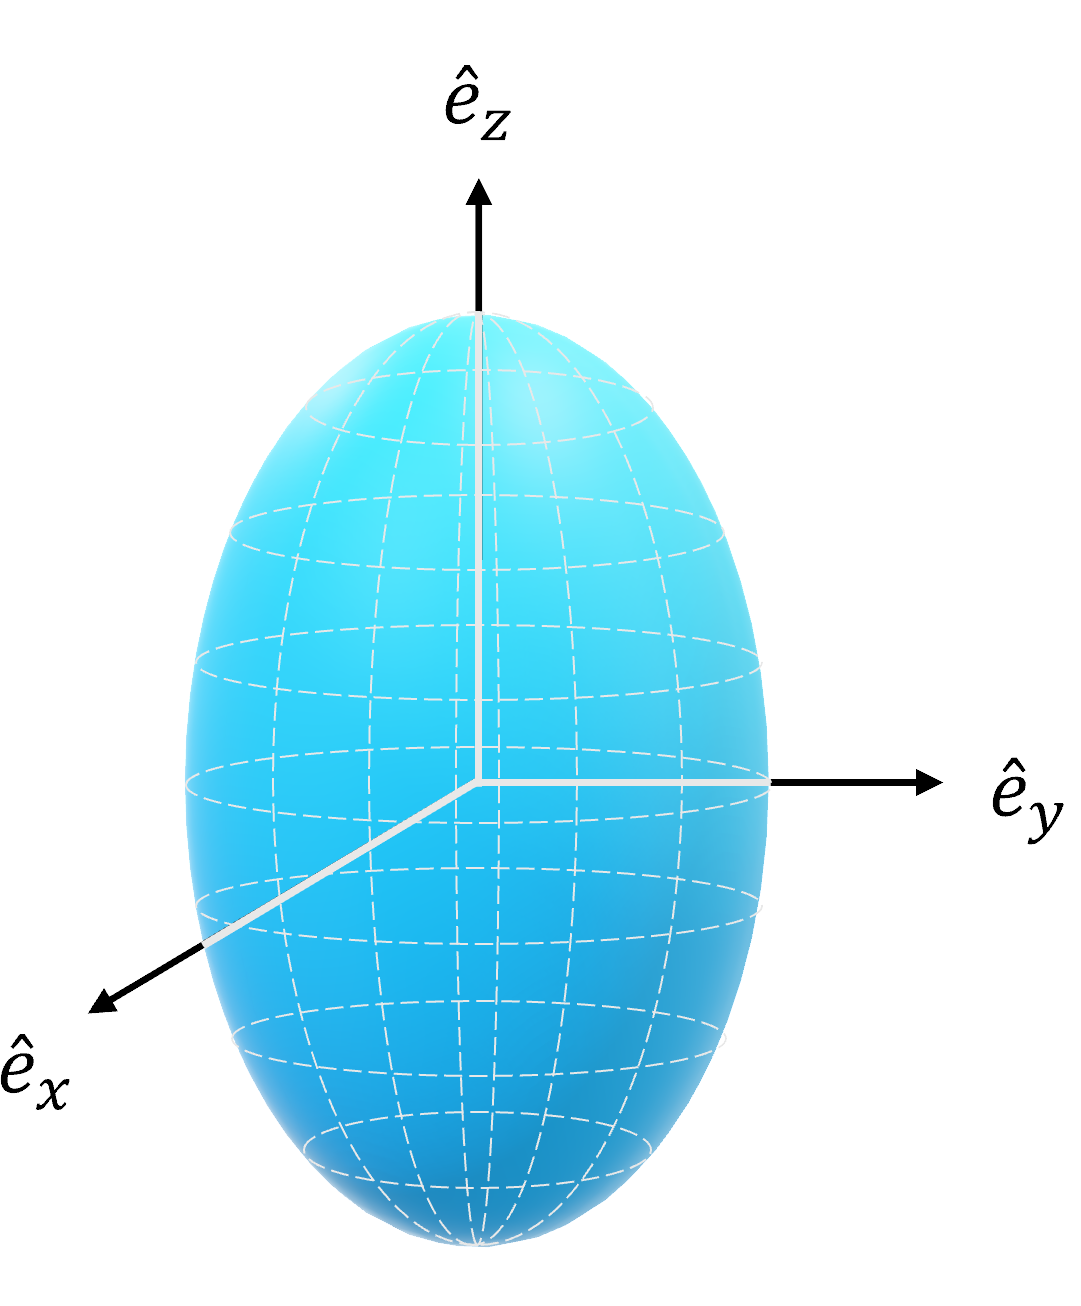
\includegraphics[width=.23\textwidth]{../../Figuras/prolato} \label{esf_prolato}}\quad%
	\sidesubfloat[]{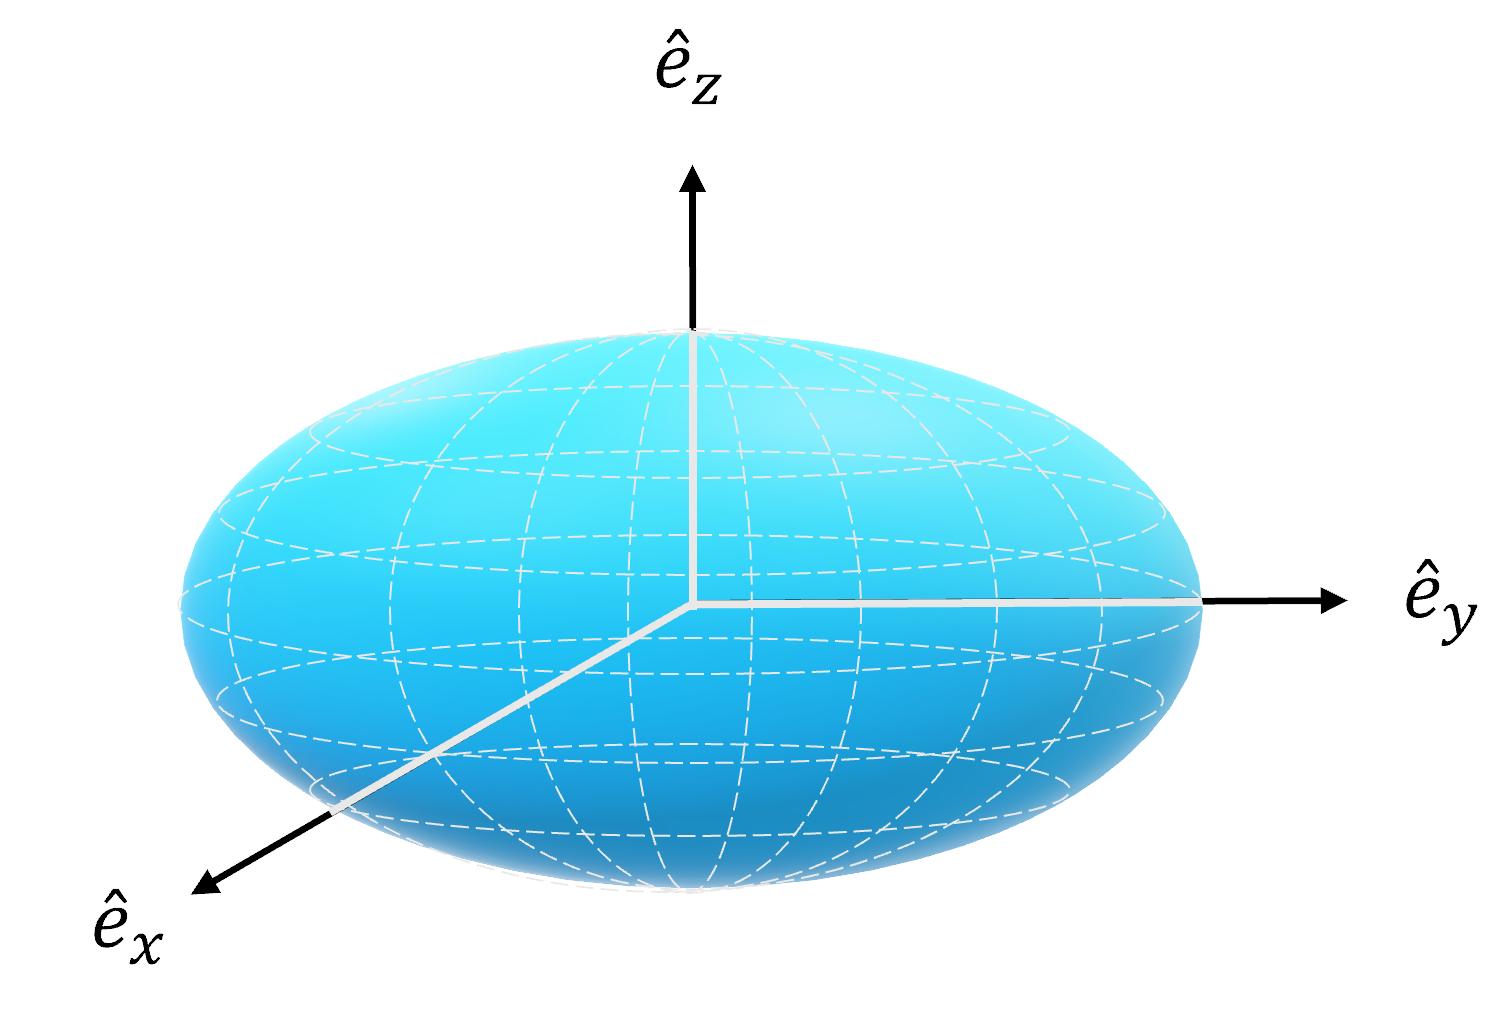
\includegraphics[width=.3\textwidth]{../../Figuras/oblato.pdf}\label{esf_oblato}}%
	\caption{Clases especiales de elipsoides. \textbf{a)} Prolato: el eje mayor del elipsoide está orientado en la dirección del eje $\hat{e}_z$. \textbf{b)} Oblato: el eje mayor del elipsoide está orientado en la dirección del eje $\hat{e}_y$.}\label{fig:test}
\end{figure}

